\section{Parser}
\label{sec:parser}
The first step of our RAM interpreter is to parse the instructions. At first we tried to use \textbf{ANTLR4}, it's a parser generator for reading, processing, executing, or translating structured text. Margaux having already used it, it seemed to be a good choice to make the parsing, but once most of the grammar was done, we had a problem.

When we wanted to add the name of the macros and each instruction was detected as a string caused by a priority action problem. Therefore, we started to seek for a solution and we found a Python library named \textbf{PLY} that was easier to use and seemed to solve our problem.

\textbf{PLY} is a Python implementation of the lex and yacc tools commonly used to write parsers and compilers. The parsing is based on the same \textbf{LALR} algorithm used by many yacc tools. \textbf{LALR} parser is a simplified version of an \textbf{LR} parser, for parsing text according to a set of production rules specified by a formal grammar for a computer language. \textbf{LR} is left-to-right derivation.

Our parser detects 10 main kind of grammar rules.

\begin{lstlisting}[
    caption={Detected instruction}, 
    label={detected_instruction},
    mathescape, 
    frame=lines,
    backgroundcolor=\color{gray!10}, breaklines=true
    ]
    0. Rk = Rk + 1
    1. Rk = Rk - 1
    2. if Rk != 0 then gotob n
    3. if Rk != 0 then gotof n
    4. push Rk
    5. pop Rk
    6. rp(Rk, Rl)
    7. lp(Rk, Rl)
    8. begin macro <name> (Rk, Rl, ..., Rz)<code> end macro;
    9. <name> (Rk, Rl, ..., Rz)
\end{lstlisting}

\subsection{Lexical analysis}
The first step of our parser is to make the lexical analyse which verifies if the used vocabulary is correct. We have decided to allow only lower case letters except for the \textbf{R} in registers which can only be capitalized.

So we detected all the words that would be useful to us in addition to the strings for the names of the macros and the numbers for the registers.

\newpage
\subsection{Syntactic analysis}

The creation of grammar \ref{grammar} took longer than expected. It syntactic analysis verifies that the arrangement of words is coherent. We had to create a redundant grammar because the instructions to be parsed in the macros and outside are very similar. For example, in macros, we can have registers with a not known value (a register with name \textbf{$R_x$} is authorized inside a macro definition but not outside).

\subsection{Semantic analysis}
The semantic analysis verifies that the instructions have a meaning else we raise an error. 

In listing \ref{semantic_rules} the number associated with the instructions is the same as in listing \ref{detected_instruction}.

\begin{lstlisting}[
    caption={Semantic rules}, 
    label={semantic_rules},
    mathescape, 
    frame=lines,
    backgroundcolor=\color{gray!10}, breaklines=true
    ]
    1. The instructions 0 and 1 must add and subtract 1.
    2. The instructions 2 and 3 must compare Rk with 0.
    3. The register list of instruction 8 must contain only "register variables"[1].
    4. The instruction 9 must have the same number of arguments as this statement.
    5. All instructions of a macro using "register variables" must be those declared in the arguments of the macro.

    [1] The variable registers are in Rstring format.
\end{lstlisting}

If one of the lexical, syntactic or semantic rules is not respected an error is raised indicating the line of the problem.

\subsection{Creation of the chained list}

All parsed instructions are translated into \textbf{Instruction} objects except for macro declarations which create \textbf{Macro} objects. \textbf{Macro} are a sub type of instruction that have the particularity to contain Instructions. When parsing the text we create a chained list with our instructions and we do the same for the \textbf{Instructions} in the \textbf{Macro}.

The Figure \ref{tree} shows the tree created from the code of Listing \ref{example_code}. The left branch represent the next Instruction and the right Instruction in the Macro.

\newpage
\begin{lstlisting}[
    caption={Example of code with macro}, 
    label={example_code},
    mathescape, 
    frame=lines,
    backgroundcolor=\color{gray!10}, breaklines=true]
begin macro clear(Rx)
    Rx = Rx - 1
    if Rx != 0 then gotob 1
end macro;
R0 = R0 + 1
clear(R0)
\end{lstlisting}


\begin{figure}[H]
    \centering
    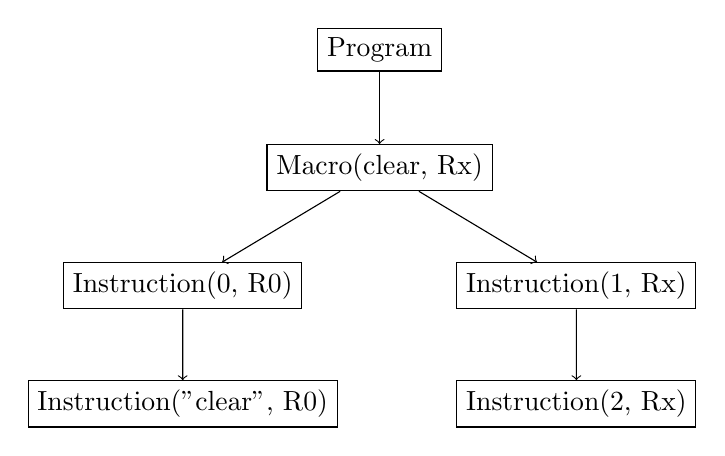
\begin{tikzpicture}[nodes={draw}, ->]

    \node{Program}[sibling distance = 5cm]
    child {node{Macro(clear, Rx)}
        child {node{Instruction(0, R0)}
            child {node{Instruction("clear", R0)}
                }}
    child { node {Instruction(1, Rx)} 
        child { node {Instruction(2, Rx)} 
            }}}
        ;
    \end{tikzpicture}
    \caption{Tree of the example code}
    \label{tree}
\end{figure}







